\setbackground
{
	\centering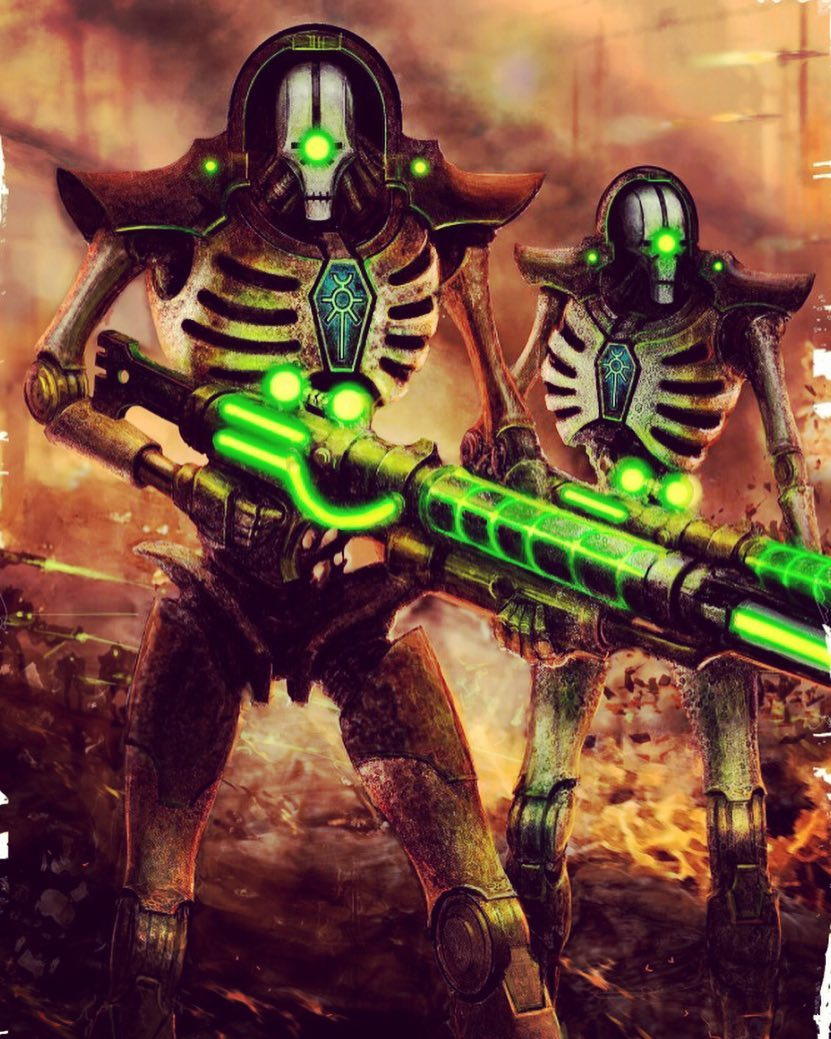
\includegraphics[height=530pt, width=400pt]{elite_art.jpg}
	\subsection[Elites]{\texorpdfstring{\centering\Huge Elite}{Elites}}
	
	\centerline{\begin{minipage}{400pt}
			\centering
		I am not capricious, nor am I given to cruel acts for their own sakes. It is simply a fact that you and your kind have trespassed, and thus invited extermination. Curse you for putting me to this inconvenience.
		
		\vspace*{1em}
		\raggedleft Anrakyr the Traveller
	\end{minipage}}
}

\newpage
\clearbackground
\subsubsection[Pariah Lychguard Phalanx]{}
\fbox{\begin{imgminipage}{marble.jpg}[t][0.90\textheight]{0.2\textwidth}
		\color{white}
		\centering {\large ELITES}
		
		\raggedright \small
		\color{black}
\end{imgminipage}}
\hspace{0.5em}
\begin{minipage}[t]{0.72\textwidth}
	{\large \textbf{Pariah Lychguard Phalanx \dotfill 175 Points}}
	
	\begin{tabular}{m{160 pt} *{10}{c}}
		& M & WS & BS & S & T & W & I & A & Ld & Sv \\
		\hline
		Pariah Lychguard & 7 & 4 & 4 & 5 & 5 & 2 & 2 & 1 & 10 & 3+ \\
	\end{tabular}
	\small
	\begin{minipage}[t]{0.5\textwidth}
		\begin{flushleft}
		\vspace*{2em}
		\textbf{Unit Composition}
		\begin{itemize}
			\item 5 Pariah Lychguard
		\end{itemize}
		
		\textbf{Wargear}
		\begin{itemize}
			\item \quickref{Warscythe}
		\end{itemize}
		\end{flushleft}
	\end{minipage}
	\begin{minipage}[t]{0.5\textwidth}
		\begin{flushleft}
		\vspace*{2em}
		\textbf{Unit Type}
		\begin{itemize}
			\item Infantry (Anathema, \quickref{Living Metal})
		\end{itemize}
		
		\textbf{Special Rules}
		\begin{itemize}
			\item \quickref{Awakening Protocols} (Bronze)
			\item Chosen Warriors
			\item Fearless
			\item \quickref{Reanimation Protocols}
			\item Shock and Awe
		\end{itemize}
		\end{flushleft}
	\end{minipage}
	
	\vspace*{2em}
	\textbf{Weapons}
	
	\begin{tabular}{L{90 pt} c C{40pt} *{2}{c} >{\raggedright\arraybackslash}p{130pt}}
		& Range & Type & S & AP & Abilities \\
		\hline
		\quickref{Hyperphase Sword} & — & Melee & User & 3 & Rending (5+) \\
		\quickref{Warscythe} & — & Melee & +2 & 2 & Armourbane (Melee), Two-Handed \\
		\quickref{Gauss Blaster} & 24" & Rapid Fire & 5 & 4 & \quickref{Gauss} (6+) \\
	\end{tabular}
	
	\vspace*{2em}
	\textbf{Unit Rules}
	
	\textit{Shock and Awe}: Pariah Lychguard ignore the Living Metal sub-type's restriction on performing Sweeping Advances.
		
	\vspace*{2em}
	\textbf{Dedicated Transport}
	A Pariah Lychguard Phalanx may take a Night Scythe as a Dedicated Transport. As a Dedicated Transport this does not use up an additional Force Organisation slot, but its points cost must still be paid for as part of the army.
	
	\vspace*{2em}
	\textbf{Options}
	\begin{itemize}
		\item The Pariah Lychguard Phalanx may include:
		\begin{itemize}
			\item Up to an additional 5 Pariah Lychguards \dotfill +35 points each
		\end{itemize}
		\item The entire unit may exchange their \quickref{Warscythe} for one of the following options:
		\begin{itemize}
			\item \quickref{Warscythe} with in-built \quickref{Gauss Blaster} \dotfill +5 points each
			\item \quickref{Hyperphase Sword} and \quickref{Dispension Shield} \dotfill +8 points each
		\end{itemize}
	\end{itemize}
\end{minipage}


\newpage
\subsubsection[Royal Lychguard Phalanx]{}
\begin{minipage}[t]{0.72\textwidth}
	{\large \textbf{Royal Lychguard Phalanx \dotfill 175 Points}}
	
	\begin{tabular}{m{160 pt} *{10}{c}}
		& M & WS & BS & S & T & W & I & A & Ld & Sv \\
		\hline
		Royal Lychguard & 7 & 4 & 4 & 5 & 5 & 2 & 2 & 2 & 10 & 3+ \\
	\end{tabular}
	\small
	\begin{minipage}[t]{0.5\textwidth}
		\begin{flushleft}
		\vspace*{2em}
		\textbf{Unit Composition}
		\begin{itemize}
			\item 5 Royal Lychguard
		\end{itemize}
		
		\textbf{Wargear}
		\begin{itemize}
			\item \quickref{Warscythe}
		\end{itemize}
		\end{flushleft}
	\end{minipage}
	\begin{minipage}[t]{0.5\textwidth}
		\begin{flushleft}
		\vspace*{2em}
		\textbf{Unit Type}
		\begin{itemize}
			\item Infantry (Line, \quickref{Living Metal})
		\end{itemize}
		
		\textbf{Special Rules}
		\begin{itemize}
			\item \quickref{Awakening Protocols} (Bronze)
			\item Chosen Warriors
			\item \quickref{Reanimation Protocols}
			\item Royal Guard
		\end{itemize}
		\end{flushleft}
	\end{minipage}
	
	\vspace*{2em}
	\textbf{Weapons}
	
	\begin{tabular}{L{90 pt} c C{40pt} *{2}{c} >{\raggedright\arraybackslash}p{130pt}}
		& Range & Type & S & AP & Abilities \\
		\hline
		\quickref{Hyperphase Sword} & — & Melee & User & 3 & Rending (5+) \\
		\quickref{Warscythe} & — & Melee & +2 & 2 & Armourbane (Melee), Two-Handed \\
		\quickref{Gauss Blaster} & 24" & Rapid Fire & 5 & 4 & \quickref{Gauss} (6+) \\
	\end{tabular}
	
	\vspace*{2em}
	\textbf{Unit Rules}
	
%	TODO: Right this with the Decurion Nemesor ability
	\textit{Royal Guard}: Only a single Royal or Charnel Lychguard Phalanx unit may be purchased for each Lord, Nemesor Lord, Nemesor Overlord, and/or Phaeron in your army list and are treated as their personal retinue. This does not use up an additional Force Organisation slot and they do not have to be deployed with them. They count as within Nodal Command Range of their respective HQ while they are both on the table. Additionally, if there are no models with the Noble sub-type attached to the Royal Lychguard Phalanx unit, the Royal Lychguard ignore the Living Metal sub-type's restriction on performing Sweeping Advances.
	
	\vspace*{2em}
	\textbf{Dedicated Transport}
	A Royal Lychguard Phalanx may take a Night Scythe as a Dedicated Transport. As a Dedicated Transport this does not use up an additional Force Organisation slot, but its points cost must still be paid for as part of the army.
	
	\vspace*{2em}
	\textbf{Options}
	\begin{itemize}
		\item The Royal Lychguard Phalanx may include:
		\begin{itemize}
			\item Up to an additional 5 Royal Lychguards \dotfill +35 points each
		\end{itemize}
		\item The entire unit may exchange their \quickref{Warscythe} for one of the following options:
		\begin{itemize}
			\item \quickref{Warscythe} with in-built \quickref{Gauss Blaster} \dotfill +5 points each
			\item \quickref{Hyperphase Sword} and \quickref{Dispersion Shield} \dotfill +8 points each
		\end{itemize}
		\item One Royal Lychguard may take:
		\begin{itemize}
			\item \quickref{Dynastic Ankh} \dotfill +10 points
		\end{itemize} 
	\end{itemize}
\end{minipage}
\hspace{0.5em}
\fbox{\begin{imgminipage}{marble.jpg}[t][0.90\textheight]{0.2\textwidth}
	\color{white}
	\centering {\large ELITES}
	
	\raggedright \small
	\color{black}
\end{imgminipage}}


\newpage
\subsubsection{Apprentek}

%TODO: This


\newpage
\subsubsection[Canoptek Cryptothrall Cohort]{}
\begin{minipage}[t]{0.72\textwidth}
	{\large \textbf{Canoptek Cryptothrall Cohort \dotfill 40 Points}}
	
	\begin{tabular}{m{160 pt} *{10}{c}}
		& M & WS & BS & S & T & W & I & A & Ld & Sv \\
		\hline
		Canoptek Cryptothrall & 6 & 3 & 3 & 5 & 5 & 1 & 2 & 2 & 10 & 3+ \\
	\end{tabular}
	\small
	\begin{minipage}[t]{0.5\textwidth}
		\begin{flushleft}
		\vspace*{2em}
		\textbf{Unit Composition}
		\begin{itemize}
			\item 2 Canoptek Cryptothralls
		\end{itemize}
		
		\textbf{Wargear}
		\begin{itemize}
			\item Close Combat Weapon
			\item \quickref{Scouring Eye}
		\end{itemize}
		\end{flushleft}
	\end{minipage}
	\begin{minipage}[t]{0.5\textwidth}
		\begin{flushleft}
		\vspace*{2em}
		\textbf{Unit Type}
		\begin{itemize}
			\item Infantry (\quickref{Canoptek}, \quickref{Living Metal})
		\end{itemize}
		
		\textbf{Special Rules}
		\begin{itemize}
			\item \quickref{Awakening Protocols} (Bronze)
			\item Bound Creation
			\item Enthralled Protector
			\item \quickref{Reanimation Protocols}
			\item \quickref{Soulless Hordes} (Bronze)
			\item Systematic Vigor
		\end{itemize}
		\end{flushleft}
	\end{minipage}
	
	\vspace*{2em}
	\textbf{Weapons}
	
	\begin{tabular}{L{90 pt} c C{40pt} *{2}{c} >{\raggedright\arraybackslash}p{130pt}}
		& Range & Type & S & AP & Abilities \\
		\hline
		\quickref{Scouring Eye} & 12" & Pistol 2 & 5 & 5 & — \\
	\end{tabular}
	
	\vspace*{2em}
	\textbf{Unit Rules}
	
	\textit{Bound Creation:} For each Cryptek or Cryptek Lord in your army, a Canoptek Cryptothrall Cohort unit can be taken without taking up a Force Org slot. This unit starts the game attached to those units.
	
	\textit{Enthralled Protector:} If a unit contains a Canoptek Cryptothrall model as well as one or more Crypteks or Cryptek Lords, any Wounds which would be allocated to the Crypteks or Cryptek Lords (even those caused by the Precision Strikes (X) or Sniper special rules) may instead be allocated to a Canoptek Cryptothrall first.
	
	\textit{Systematic Vigor:} If a Canoptek Cryptothrall is in a unit with a Cryptek or Cryptek Lord, increase its BS, WS, and A to 4.
\end{minipage}
\hspace{0.5em}
\fbox{\begin{imgminipage}{marble.jpg}[t][0.90\textheight]{0.2\textwidth}
		\color{white}
		\centering {\large ELITES}
		
		\raggedright \small
		\color{black}
\end{imgminipage}}


\newpage
\subsubsection[Canoptek Plasmacyte]{}
\begin{minipage}[t]{0.72\textwidth}
	{\large \textbf{Canoptek Plasmacyte \dotfill 15 Points}}
	
	\begin{tabular}{m{160 pt} *{10}{c}}
		& M & WS & BS & S & T & W & I & A & Ld & Sv \\
		\hline
		Canoptek Plasmacyte & 9 & 3 & 3 & 4 & 5 & 1 & 2 & 1 & 10 & 4+ \\
	\end{tabular}
	\small
	\begin{minipage}[t]{0.5\textwidth}
		\begin{flushleft}
		\vspace*{2em}
		\textbf{Unit Composition}
		\begin{itemize}
			\item 1 Canoptek Plasmacyte
		\end{itemize}
		
		\textbf{Wargear}
		\begin{itemize}
			\item Close Combat Weapon
		\end{itemize}
		\end{flushleft}
	\end{minipage}
	\begin{minipage}[t]{0.5\textwidth}
		\begin{flushleft}
		\vspace*{2em}
		\textbf{Unit Type}
		\begin{itemize}
			\item Infantry (\quickref{Canoptek}, Floating, \quickref{Living Metal})
		\end{itemize}
		
		\textbf{Special Rules}
		\begin{itemize}
			\item \quickref{Awakening Protocols} (Bronze)
			\item Engram Specialization
			\item \quickref{Reanimation Protocols}
			\item Metasentient Energization
			\item Viral Construct
		\end{itemize}
		\end{flushleft}
	\end{minipage}
		
	\vspace*{2em}
	\textbf{Unit Rules}
	
	\textit{Engram Specialization}: When taking a Canoptek Plasmacyte model, you must select a specialization: Destructor, Accelerator, or Reanimator. This determines the effects of the model's Metasentient Energization special rule. 
	
	\textit{Metasentient Energization (Destructor):} Once per turn at the start of the Assault Phase, all other models with the Destroyer sub-type in the Plasmacyte's attached unit gains +1 S and +1 A until the end of the turn. If you do so, roll a D6: on a 5+, the unit suffers an immediate Wound, which only Invulnerable Saves and Damage Mitigation rolls can prevent.
	
	\textit{Metasentient Energization (Accelerator):} Once per turn, after the Plasmacyte or its attached unit fails a Leadership test, you may have the unit re-roll the check. If you do so, roll a D6: on a 5+, the unit suffers an immediate Wound, which only Invulnerable Saves and Damage Mitigation rolls can prevent.
	
	\textit{Metasentient Energization (Reanimator):} Once per turn, when the Plasmacyte or its attached unit's \quickref{Reanimation Protocols} is triggered, you may add a +1 to all the reanimate rolls. If you do so, roll a D6: on a 4+, the unit suffers an immediate Wound, which only Invulnerable Saves and Damage Mitigation rolls can prevent. Each unit can only ever be affected by one Plasmacyte Reanimator each turn.
	
	\textit{Viral Construct:} For each unit with the Destroyer sub-type in your army, a Canoptek Plasmacyte Destructor may be taken without taking up a Force Organization slot. For each Cryptek or Cryptek Lord in your army, a Canoptek Plasmacyte Accelerator or Canoptek Plasmacyte Reanimator can be taken without taking up a Force Organization slot. This unit starts the game attached to those units. 
\end{minipage}
\hspace{0.5em}
\fbox{\begin{imgminipage}{marble.jpg}[t][0.90\textheight]{0.2\textwidth}
		\color{white}
		\centering {\large ELITES}
		
		\raggedright \small
		\color{black}
\end{imgminipage}}


\newpage
\subsubsection[Canoptek Reanimator]{}

\fbox{\begin{imgminipage}{marble.jpg}[t][0.90\textheight]{0.2\textwidth}
		\color{white}
		\centering {\large ELITES}
		
		\raggedright \small
		\color{black}
\end{imgminipage}}
\hspace{0.5em}
\begin{minipage}[t]{0.72\textwidth}
	{\large \textbf{Canoptek Reanimator \dotfill 70 Points}}
	
	\begin{tabular}{m{160 pt} *{10}{c}}
		& M & WS & BS & S & T & W & I & A & Ld & Sv \\
		\hline
		Canoptek Reanimator & 8 & 3 & 3 & 5 & 5 & 4 & 2 & 4 & 10 & 3+ \\
	\end{tabular}
	\small
	\begin{minipage}[t]{0.5\textwidth}
		\begin{flushleft}
		\vspace*{2em}
		\textbf{Unit Composition}
		\begin{itemize}
			\item 1 Canoptek Reanimator
		\end{itemize}
		
		\textbf{Wargear}
		\begin{itemize}
			\item \quickref{Atomiser Beam Lance}
			\item Close Combat Weapon
		\end{itemize}
		\end{flushleft}
	\end{minipage}
	\begin{minipage}[t]{0.5\textwidth}
		\begin{flushleft}
		\vspace*{2em}
		\textbf{Unit Type}
		\begin{itemize}
			\item Dreadnought (\quickref{Canoptek}, Floating, \quickref{Living Metal})
		\end{itemize}
	
		
		\textbf{Special Rules}
		\begin{itemize}
			\item \quickref{Awakening Protocols} (Bronze)
			\item \quickref{Reanimation Protocols}
			\item Nanoscarab Reanimation Beam
		\end{itemize}
		\end{flushleft}
	\end{minipage}
	
	
	\vspace*{2em}
	\textbf{Weapons}
	
	\begin{tabular}{L{90 pt} c C{40pt} *{2}{c} >{\raggedright\arraybackslash}p{130pt}}
		& Range & Type & S & AP & Abilities \\
		\hline
		\quickref{Atomiser Beam Lance} & 12" & Heavy 3 & 6 & 4 & Murderous Strike (6+) \\
	\end{tabular}

	\vspace*{2em}
	\textbf{Unit Rules}
	
	\textit{Nanoscarab Reanimation Beam}: At the start of your Movement phase you may select one friendly unit with the \quickref{Reanimation Protocols} special rule. Until your next turn, while that unit is within 6" of this model and visibile to it, add a +1 to all \quickref{Reanimation Protocols} rolls. Each unit can only ever be targeted by one Reanimation Beam at a time.
\end{minipage}


\newpage
\subsubsection[Deathmark Squadron]{}
\begin{minipage}[t]{0.72\textwidth}
	{\large \textbf{Deathmark Squadron \dotfill 70 Points}}
	
	\begin{tabular}{m{160 pt} *{10}{c}}
		& M & WS & BS & S & T & W & I & A & Ld & Sv \\
		\hline
		Deathmark & 6 & 4 & 4 & 5 & 5 & 1 & 2 & 2 & 10 & 3+ \\
	\end{tabular}
	\small
	\begin{minipage}[t]{0.5\textwidth}
		\begin{flushleft}
		\vspace*{2em}
		\textbf{Unit Composition}
		\begin{itemize}
			\item 5 Deathmarks
		\end{itemize}
		
		\textbf{Wargear}
		\begin{itemize}
			\item \quickref{Synaptic Disintegrator}
		\end{itemize}
		\end{flushleft}
	\end{minipage}
	\begin{minipage}[t]{0.5\textwidth}
		\begin{flushleft}
		\vspace*{2em}
		\textbf{Unit Type}
		\begin{itemize}
			\item Infantry (\quickref{Living Metal})
		\end{itemize}
		
		\textbf{Special Rules}
		\begin{itemize}
			\item \quickref{Awakening Protocols} (Bronze)
			\item Deep-Strike
			\item \quickref{Ethereal Interceptors}
			\item \quickref{Reanimation Protocols}
			\item Hyperspace Ambush
			\item \quickref{Hyperspace Hunters}
			\item Marked for Death
		\end{itemize}
		\end{flushleft}
	\end{minipage}
	
	\vspace*{2em}
	\textbf{Weapons}
	
	\begin{tabular}{L{90 pt} c C{40pt} *{2}{c} >{\raggedright\arraybackslash}p{130pt}}
		& Range & Type & S & AP & Abilities \\
		\hline
		\quickref{Synaptic Disintegrator} & 36" & Rapid Fire & 5 & 5 & Rending (5+), Pinning, Sniper \\
	\end{tabular}
	
	\vspace*{2em}
	\textbf{Unit Rules}
	
	\textit{Hyperspace Ambush:}  During the player turn in which this unit arrives from Deep Strike Reserve, all shooting attacks made by the Deathmarks in this unit will wound on To Wound rolls of 2+, regardless of the victim’s Toughness.
	
	\vspace*{2em}
	\textbf{Dedicated Transport}
	A Deathmark Squadron may take a Night Scythe as a Dedicated Transport. As a Dedicated Transport this does not use up an additional Force Organisation slot, but its points cost must still be paid for as part of the army.
	
	\vspace*{2em}
	\textbf{Options}
	\begin{itemize}
		\item The Deathmark Squadron may include:
		\begin{itemize}
			\item Up to an additional 5 Deathmarks \dotfill +14 points each
		\end{itemize}
		\item The entire unit may take any of the following options:
		\begin{itemize}
			\item \quickref{Hyper-Oubliette Navigator} \dotfill +5 points each
		\end{itemize}
	\end{itemize}
\end{minipage}
\hspace{0.5em}
\fbox{\begin{imgminipage}{marble.jpg}[t][0.90\textheight]{0.2\textwidth}
		\color{white}
		\centering {\large ELITES}
		
		\raggedright \small
		\color{black}
\end{imgminipage}}


\newpage
\subsubsection[C'tan Shard of Aza'gorod, the Nightbringer]{}

\fbox{\begin{imgminipage}{marble.jpg}[t][0.90\textheight]{0.2\textwidth}
		\color{white}
		\centering {\large ELITES}
		
		\raggedright \small
		\color{black}
\end{imgminipage}}
\hspace{0.5em}
\begin{minipage}[t]{0.72\textwidth}
	{\large \textbf{C'tan Shard of Aza'gorod, the Nightbringer \dotfill 330 Points}}
	
	\begin{tabular}{m{160 pt} *{10}{c}}
		& M & WS & BS & S & T & W & I & A & Ld & Sv \\
		\hline
		Nightbringer & 9 & 6 & 4 & 7 & 7 & 5 & 4 & 4 & 10 & 4+ \\
	\end{tabular}
	\small
	\begin{minipage}[t]{0.5\textwidth}
		\begin{flushleft}
		\vspace*{2em}
		\textbf{Unit Composition}
		\begin{itemize}
			\item 1 Nightbringer
		\end{itemize}
		
		\textbf{Wargear}
		\begin{itemize}
			\item \quickref{Scythe of the Nightbringer}
		\end{itemize}
		\end{flushleft}
	\end{minipage}
	\begin{minipage}[t]{0.5\textwidth}
		\begin{flushleft}
		\vspace*{2em}
		\textbf{Unit Type}
		\begin{itemize}
			\item Infantry (\quickref{C'Tan})
		\end{itemize}
		
		\textbf{Special Rules}
		\begin{itemize}
			\item \quickref{Awakening Protocols} (Silver)
			\item Bulky (5)
			\item \quickref{Drain Life}
			\item Enslaved Star God
			\item Eternal Warrior
			\item Fearless
			\item Immune to Natural Laws
			\item Necrodermis Vessel
			\item Night Vision
			\item Powers of the C'tan
			\item \quickref{Reanimation Protocols}
		\end{itemize}
		\end{flushleft}
	\end{minipage}
	
	\vspace*{2em}
	\textbf{Weapons}
	
	\begin{tabular}{L{90 pt} c C{40pt} *{2}{c} >{\raggedright\arraybackslash}p{130pt}}
		& Range & Type & S & AP & Abilities \\
		\hline
		Scythe of the Nightbringer & & & & & \\
		— Reaping Sweep & — & Melee & User & 3 & Murderous Strike (6+), Reaping Blow (4) \\
		— Entropic Blow & — & Melee & x2 & 2 & Brutal (3), Murderous Strike (5+), Two-Handed \\
	\end{tabular}
	
	\vspace*{2em}
	\textbf{Unit Rules}
		
	\textit{Enslaved Star God}: If this model would be removed (after \quickref{Reanimation Protocols} roll have been failed), roll a D6. On a 1, the shackles of the C'tan Shard have been broken and it is now \textit{rampaging}. The opposing player returns the model to a point within 3" of where it dies with 1 Wound remaining. While rampaging, the C'tan Shard is considered an enemy unit to all players and takes its turns at the beginning of its owner's turns use the standard rules. It will attempt to attack the closest and highest number of units possible each turn, preferring its owner's units in case of a tie. If it would be removed while rampaging, this ability does not trigger again.
	
	\textit{Immune to Natural Laws:} When moving, this model can move over all other models and terrain freely, and automatically passes Dangerous Terrain tests. However, it cannot end its move on top of other models and can only end its move on top of impassable terrain if it is possible to actually place the model on top of it.
	
	\textit{Necrodermis Vessel:} The C'tan has a 4+ invulnerable save and ignores the Living Metal sub-type's restriction on performing Sweeping Advances.
	
	\textit{Powers of the C'tan:} The Nightbringer has two C'tan Powers at the Shard Level. One is the \quickref{Gaze of Death} specialty power, and the other must be chosen below.
	
	\vspace*{2em}
	\textbf{Options}
	\begin{itemize}
		\item The Nightbringer chooses a second power from the following options:
		\begin{itemize}
			\item \quickref{Antimatter Meteor} \dotfill X pt
			\item \quickref{Cosmic Fire} \dotfill X pt
			\item \quickref{Entropic Touch} \dotfill X pt
			\item \quickref{Moulder of Worlds} \dotfill X pt
			\item \quickref{Pyreshards} \dotfill X pt
			\item \quickref{Sentient Singularity} \dotfill X pt
			\item \quickref{Seismic Assault} \dotfill X pt
			\item \quickref{Sky of Falling Stars} \dotfill X pt
			\item \quickref{Swarm of Spirit Dust} \dotfill X pt
			\item \quickref{Time's Arrow} \dotfill X pt
			\item \quickref{Transdimensional Thunderbolt} \dotfill X pt
			\item \quickref{Withering Worldscape} \dotfill X pt
		\end{itemize}
	\end{itemize}
\end{minipage}



\newpage
\subsubsection[C'tan Shard of Mephet'ran, the Deceiver]{}

\begin{minipage}[t]{0.72\textwidth}
	{\large \textbf{C'tan Shard of Mephet'ran, the Deceiver \dotfill 280 Points}}
	
	\begin{tabular}{m{160 pt} *{10}{c}}
		& M & WS & BS & S & T & W & I & A & Ld & Sv \\
		\hline
		Deceiver & 9 & 5 & 5 & 7 & 7 & 5 & 4 & 4 & 10 & 4+ \\
	\end{tabular}
	\small
	\begin{minipage}[t]{0.5\textwidth}
		\begin{flushleft}
		\vspace*{2em}
		\textbf{Unit Composition}
		\begin{itemize}
			\item 1 Deceiver
		\end{itemize}
		
		\textbf{Wargear}
		\begin{itemize}
			\item \quickref{Golden Fists}
		\end{itemize}
		\end{flushleft}
	\end{minipage}
	\begin{minipage}[t]{0.5\textwidth}
		\begin{flushleft}
		\vspace*{2em}
		\textbf{Unit Type}
		\begin{itemize}
			\item Infantry (\quickref{C'Tan})
		\end{itemize}
		
		\textbf{Special Rules}
		\begin{itemize}
			\item \quickref{Awakening Protocols} (Silver)
			\item Bulky (5)
			\item Enslaved Star God
			\item Eternal Warrior
			\item Fearless
			\item Immune to Natural Laws
			\item \quickref{Misdirection}
			\item Necrodermis Vessel
			\item Night Vision
			\item Powers of the C'tan
			\item \quickref{Reanimation Protocols}
		\end{itemize}
		\end{flushleft}
	\end{minipage}
	
	\vspace*{2em}
	\textbf{Weapons}
	
	\begin{tabular}{L{90 pt} c C{40pt} *{2}{c} >{\raggedright\arraybackslash}p{130pt}}
		& Range & Type & S & AP & Abilities \\
		\hline
		Golden Fists & — & Melee & User & 3 & Brutal (2) \\
	\end{tabular}
	
	\vspace*{2em}
	\textbf{Unit Rules}
	
	\textit{Enslaved Star God}: If this model would be removed (after \quickref{Reanimation Protocols} roll have been failed), roll a D6. On a 1, the shackles of the C'tan Shard have been broken and it is now \textit{rampaging}. The opposing player returns the model to a point within 3" of where it dies with 1 Wound remaining. While rampaging, the C'tan Shard is considered an enemy unit to all players and takes its turns at the beginning of its owner's turns use the standard rules. It will attempt to attack the closest and highest number of units possible each turn, preferring its owner's units in case of a tie. If it would be removed while rampaging, this ability does not trigger again.
	
	\textit{Immune to Natural Laws:} When moving, this model can move over all other models and terrain freely, and automatically passes Dangerous Terrain tests. However, it cannot end its move on top of other models and can only end its move on top of impassable terrain if it is possible to actually place the model on top of it.
		
	\textit{Necrodermis Vessel:} The Deceiver has a 4+ invulnerable save and ignores the Living Metal sub-type's restriction on performing Sweeping Advances.
	
	\textit{Powers of the C'tan:} The Deceiver has two C'tan Powers at the Shard Level. One is the \quickref{Grand Illusion} specialty power, and the other must be chosen below.
	
	\vspace*{2em}
	\textbf{Options}
	\begin{itemize}
		\item The Deceiver chooses a second power from the following options:
		\begin{itemize}
			\item \quickref{Antimatter Meteor} \dotfill X pt
			\item \quickref{Cosmic Fire} \dotfill X pt
			\item \quickref{Entropic Touch} \dotfill X pt
			\item \quickref{Moulder of Worlds} \dotfill X pt
			\item \quickref{Pyreshards} \dotfill X pt
			\item \quickref{Sentient Singularity} \dotfill X pt
			\item \quickref{Seismic Assault} \dotfill X pt
			\item \quickref{Sky of Falling Stars} \dotfill X pt
			\item \quickref{Swarm of Spirit Dust} \dotfill X pt
			\item \quickref{Time's Arrow} \dotfill X pt
			\item \quickref{Transdimensional Thunderbolt} \dotfill X pt
			\item \quickref{Withering Worldscape} \dotfill X pt
		\end{itemize}
	\end{itemize}
\end{minipage}
\hspace{0.5em}
\fbox{\begin{imgminipage}{marble.jpg}[t][0.90\textheight]{0.2\textwidth}
		\color{white}
		\centering {\large ELITES}
		
		\raggedright \small
		\color{black}
\end{imgminipage}}

\newpage
\subsubsection[C'tan Shard of Mag'ladroth, the Void Dragon]{}

\fbox{\begin{imgminipage}{marble.jpg}[t][0.90\textheight]{0.2\textwidth}
		\color{white}
		\centering {\large ELITES}
		
		\raggedright \small
		\color{black}
\end{imgminipage}}
\hspace{0.5em}
\begin{minipage}[t]{0.72\textwidth}
	{\large \textbf{C'tan Shard of Mag'ladroth, the Void Dragon \dotfill 305 Points}}
	
	\begin{tabular}{m{160 pt} *{10}{c}}
		& M & WS & BS & S & T & W & I & A & Ld & Sv \\
		\hline
		Void Dragon & 9 & 5 & 5 & 7 & 7 & 5 & 4 & 4 & 10 & 4+ \\
	\end{tabular}
	\small
	\begin{minipage}[t]{0.5\textwidth}
		\vspace*{2em}
		\begin{flushleft}
		\textbf{Unit Composition}
		\begin{itemize}
			\item 1 Void Dragon
		\end{itemize}
		
		\textbf{Wargear}
		\begin{itemize}
			\item \quickref{Spear of the Void Dragon}
		\end{itemize}
		\end{flushleft}
	\end{minipage}
	\begin{minipage}[t]{0.5\textwidth}
		\vspace*{2em}
		\begin{flushleft}
		\textbf{Unit Type}
		\begin{itemize}
			\item Infantry (\quickref{C'Tan})
		\end{itemize}
		
		\textbf{Special Rules}
		\begin{itemize}
			\item \quickref{Awakening Protocols} (Silver)
			\item Bulky (9)
			\item Enslaved Star God
			\item Eternal Warrior
			\item Fearless
			\item Hammer of Wrath (2)
			\item Immune to Natural Laws
			\item \quickref{Matter Absorption}
			\item Necrodermis Vessel
			\item Night Vision
			\item Powers of the C'tan
			\item Preferred Enemy (Vehicles and Dreadnoughts)
			\item \quickref{Reanimation Protocols}
		\end{itemize}
		\end{flushleft}
	\end{minipage}
	
	\vspace*{2em}
	\textbf{Weapons}
	
	\begin{tabular}{L{90 pt} c C{40pt} *{2}{c} >{\raggedright\arraybackslash}p{130pt}}
		& Range & Type & S & AP & Abilities \\
		\hline
		Spear of the Void Dragon & & & & & \\
		— Shooting & 12" & Heavy 1 & 9 & 1 & Exoshock (5+), Lance, Line, Torsion Crusher \\
		— Melee & — & Melee & +3 & 1 & Exoshock (4+), Lance, Torsion Crusher, Two-Handed \\
	\end{tabular}
	
	\vspace*{2em}
	\textbf{Unit Rules}
	
	\textit{Enslaved Star God}: If this model would be removed (after \quickref{Reanimation Protocols} roll have been failed), roll a D6. On a 1, the shackles of the C'tan Shard have been broken and it is now \textit{rampaging}. The opposing player returns the model to a point within 3" of where it dies with 1 Wound remaining. While rampaging, the C'tan Shard is considered an enemy unit to all players and takes its turns at the beginning of its owner's turns use the standard rules. It will attempt to attack the closest and highest number of units possible each turn, preferring its owner's units in case of a tie. If it would be removed while rampaging, this ability does not trigger again.
	
	\textit{Immune to Natural Laws:} When moving, this model can move over all other models and terrain freely, and automatically passes Dangerous Terrain tests. However, it cannot end its move on top of other models and can only end its move on top of impassable terrain if it is possible to actually place the model on top of it.
		
	\textit{Necrodermis Vessel:} The Void Dragon has a 4+ invulnerable save and ignores the Living Metal sub-type's restriction on performing Sweeping Advances.
	
	\textit{Powers of the C'tan:} The Void Dragon has two C'tan Powers at the Shard Level. One is the \quickref{Voltaic Storm} specialty power, and the other must be chosen below.
	
	\vspace*{2em}
	\textbf{Options}
	\begin{itemize}
		\item The Void Dragon chooses a second power from the following options:
		\begin{itemize}
			\item \quickref{Antimatter Meteor} \dotfill X pt
			\item \quickref{Cosmic Fire} \dotfill X pt
			\item \quickref{Entropic Touch} \dotfill X pt
			\item \quickref{Moulder of Worlds} \dotfill X pt
			\item \quickref{Pyreshards} \dotfill X pt
			\item \quickref{Sentient Singularity} \dotfill X pt
			\item \quickref{Seismic Assault} \dotfill X pt
			\item \quickref{Sky of Falling Stars} \dotfill X pt
			\item \quickref{Swarm of Spirit Dust} \dotfill X pt
			\item \quickref{Time's Arrow} \dotfill X pt
			\item \quickref{Transdimensional Thunderbolt} \dotfill X pt
			\item \quickref{Withering Worldscape} \dotfill X pt
		\end{itemize}
	\end{itemize}
\end{minipage}



\newpage
\subsubsection[C'tan Shard of Nyadra'zatha, the Burning One]{}

\begin{minipage}[t]{0.72\textwidth}
	{\large \textbf{C'tan Shard of Nyadra'zatha, the Burning One \dotfill 330 Points}}
	
	\begin{tabular}{m{160 pt} *{10}{c}}
		& M & WS & BS & S & T & W & I & A & Ld & Sv \\
		\hline
		Burning One & 9 & 4 & 6 & 7 & 7 & 5 & 4 & 4 & 10 & 4+ \\
	\end{tabular}
	\small
	\begin{minipage}[t]{0.5\textwidth}
		\vspace*{2em}
		\begin{flushleft}
			\textbf{Unit Composition}
			\begin{itemize}
				\item 1 Burning One
			\end{itemize}
			
			\textbf{Wargear}
			\begin{itemize}
				\item \quickref{Voidflame Fists}
			\end{itemize}
		\end{flushleft}
	\end{minipage}
	\begin{minipage}[t]{0.5\textwidth}
		\vspace*{2em}
		\begin{flushleft}
			\textbf{Unit Type}
			\begin{itemize}
				\item Infantry (\quickref{C'Tan})
			\end{itemize}
			
			\textbf{Special Rules}
			\begin{itemize}
				\item \quickref{Awakening Protocols} (Silver)
				\item Bulky (5)
				\item Enslaved Star God
				\item Eternal Warrior
				\item Fearless
				\item \quickref{Flaming Vessel}
				\item Immune to Natural Laws
				\item Necrodermis Vessel
				\item Night Vision
				\item Powers of the C'tan
				\item Preferred Enemy (Vehicles and Dreadnoughts)
				\item \quickref{Reanimation Protocols}
			\end{itemize}
		\end{flushleft}
	\end{minipage}
	
	\vspace*{2em}
	\textbf{Weapons}
	
	\begin{tabular}{L{90 pt} c C{40pt} *{2}{c} >{\raggedright\arraybackslash}p{130pt}}
		& Range & Type & S & AP & Abilities \\
		\hline
		Voidflame Fists & — & Melee & +1 & 2 & Armourbane (Melee) \\
	\end{tabular}
	
	\vspace*{2em}
	\textbf{Unit Rules}
	
	\textit{Enslaved Star God}: If this model would be removed (after \quickref{Reanimation Protocols} roll have been failed), roll a D6. On a 1, the shackles of the C'tan Shard have been broken and it is now \textit{rampaging}. The opposing player returns the model to a point within 3" of where it dies with 1 Wound remaining. While rampaging, the C'tan Shard is considered an enemy unit to all players and takes its turns at the beginning of its owner's turns use the standard rules. It will attempt to attack the closest and highest number of units possible each turn, preferring its owner's units in case of a tie. If it would be removed while rampaging, this ability does not trigger again.
		
	\textit{Immune to Natural Laws:} When moving, this model can move over all other models and terrain freely, and automatically passes Dangerous Terrain tests. However, it cannot end its move on top of other models and can only end its move on top of impassable terrain if it is possible to actually place the model on top of it.
	
	\textit{Necrodermis Vessel:} The Burning One has a 4+ invulnerable save and ignores the Living Metal sub-type's restriction on performing Sweeping Advances.
	
	\textit{Powers of the C'tan:} The Burning One has two C'tan Powers at the Shard Level. One is the \quickref{Lord of Fire} specialty power, and the other must be chosen below.
	
	\vspace*{2em}
	\textbf{Options}
	\begin{itemize}
		\item The Void Dragon chooses a second power from the following options:
		\begin{itemize}
			\item \quickref{Antimatter Meteor} \dotfill X pt
			\item \quickref{Cosmic Fire} \dotfill X pt
			\item \quickref{Entropic Touch} \dotfill X pt
			\item \quickref{Moulder of Worlds} \dotfill X pt
			\item \quickref{Pyreshards} \dotfill X pt
			\item \quickref{Sentient Singularity} \dotfill X pt
			\item \quickref{Seismic Assault} \dotfill X pt
			\item \quickref{Sky of Falling Stars} \dotfill X pt
			\item \quickref{Swarm of Spirit Dust} \dotfill X pt
			\item \quickref{Time's Arrow} \dotfill X pt
			\item \quickref{Transdimensional Thunderbolt} \dotfill X pt
			\item \quickref{Withering Worldscape} \dotfill X pt
		\end{itemize}
	\end{itemize}
\end{minipage}
\hspace{0.5em}
\fbox{\begin{imgminipage}{marble.jpg}[t][0.90\textheight]{0.2\textwidth}
	\color{white}
	\centering {\large ELITES}
	
	\raggedright \small
	\color{black}
\end{imgminipage}}


\newpage
\subsubsection[C'tan Shard of Tsara'noga, the Outsider]{}

\fbox{\begin{imgminipage}{marble.jpg}[t][0.90\textheight]{0.2\textwidth}
		\color{white}
		\centering {\large ELITES}
		
		\raggedright \small
		\color{black}
\end{imgminipage}}
\hspace{0.5em}
\begin{minipage}[t]{0.72\textwidth}
	{\large \textbf{C'tan Shard of Tsara'noga, the Outsider \dotfill 410 Points}}
	
	\begin{tabular}{m{160 pt} *{10}{c}}
		& M & WS & BS & S & T & W & I & A & Ld & Sv \\
		\hline
		Outsider & 9 & 4 & 6 & 7 & 7 & 5 & 4 & 4 & 10 & 4+ \\
	\end{tabular}
	\small
	\begin{minipage}[t]{0.5\textwidth}
		\vspace*{2em}
		\begin{flushleft}
			\textbf{Unit Composition}
			\begin{itemize}
				\item 1 Outsider
			\end{itemize}
			
			\textbf{Wargear}
			\begin{itemize}
				\item \quickref{Touch of Eternity}
			\end{itemize}
		\end{flushleft}
	\end{minipage}
	\begin{minipage}[t]{0.5\textwidth}
		\vspace*{2em}
		\begin{flushleft}
			\textbf{Unit Type}
			\begin{itemize}
				\item Infantry (\quickref{C'Tan})
			\end{itemize}
			
			\textbf{Special Rules}
			\begin{itemize}
				\item \quickref{Awakening Protocols} (Silver)
				\item Bulky (9)
				\item Enslaved Star God
				\item Eternal Warrior
				\item Fearless
				\item Immune to Natural Laws
				\item Necrodermis Vessel
				\item Night Vision
				\item Powers of the C'tan
				\item \quickref{Reanimation Protocols}
				\item \quickref{Unfathomable Horror}
			\end{itemize}
		\end{flushleft}
	\end{minipage}
	
	\vspace*{2em}
	\textbf{Weapons}
	
	\begin{tabular}{L{90 pt} c C{40pt} *{2}{c} >{\raggedright\arraybackslash}p{130pt}}
		& Range & Type & S & AP & Abilities \\
		\hline
		Touch of Eternity & — & Melee & 10 & 1 & \quickref{Shroud of Despair} \\
	\end{tabular}
	
	\vspace*{2em}
	\textbf{Unit Rules}
	
	\textit{Enslaved Star God}: If this model would be removed (after \quickref{Reanimation Protocols} roll have been failed), roll a D6. On a 1, the shackles of the C'tan Shard have been broken and it is now \textit{rampaging}. The opposing player returns the model to a point within 3" of where it dies with 1 Wound remaining. While rampaging, the C'tan Shard is considered an enemy unit to all players and takes its turns at the beginning of its owner's turns use the standard rules. It will attempt to attack the closest and highest number of units possible each turn, preferring its owner's units in case of a tie. If it would be removed while rampaging, this ability does not trigger again.
	
	\textit{Immune to Natural Laws:} When moving, this model can move over all other models and terrain freely, and automatically passes Dangerous Terrain tests. However, it cannot end its move on top of other models and can only end its move on top of impassable terrain if it is possible to actually place the model on top of it.
	
	\textit{Necrodermis Vessel:} The Outsider has a 4+ invulnerable save and ignores the Living Metal sub-type's restriction on performing Sweeping Advances.
		
	\textit{Powers of the C'tan:} The Outsider has two C'tan Powers at the Shard Level. One is the \quickref{Gaze of the Abyss} specialty power, and the other must be chosen below.
		
	\vspace*{2em}
	\textbf{Options}
	\begin{itemize}
		\item The Outsider chooses a second power from the following options:
		\begin{itemize}
			\item \quickref{Antimatter Meteor} \dotfill X pt
			\item \quickref{Cosmic Fire} \dotfill X pt
			\item \quickref{Entropic Touch} \dotfill X pt
			\item \quickref{Moulder of Worlds} \dotfill X pt
			\item \quickref{Pyreshards} \dotfill X pt
			\item \quickref{Sentient Singularity} \dotfill X pt
			\item \quickref{Seismic Assault} \dotfill X pt
			\item \quickref{Sky of Falling Stars} \dotfill X pt
			\item \quickref{Swarm of Spirit Dust} \dotfill X pt
			\item \quickref{Time's Arrow} \dotfill X pt
			\item \quickref{Transdimensional Thunderbolt} \dotfill X pt
			\item \quickref{Withering Worldscape} \dotfill X pt
		\end{itemize}
	\end{itemize}
\end{minipage}




